%!TeX program = xelatex
\documentclass[15pt,parskip=full,a4paper]{book}
\usepackage{graphicx} 
\usepackage{parskip}
% set the default code style
\usepackage{array}
\newcolumntype{L}{>{\centering\arraybackslash}m{3cm}}
\usepackage[inner=3.7cm,outer=3.7cm]{geometry}
\begin{document}
	\chapter{Articles}
	\section{ Image processing method to determine surface area and volume of axi-symmetric agricultural products}
Knowledge of surface area of agricultural products is required as an integral part in heat and mass transfer calculations and in determination of physical properties such as gas permeability, weight per unit surface area,and respiration rates. Theoretical estimations based on a product principal dimensions and weights were investigated for eggs,[1]apples, pears and plums,[2]and apples, carrots, oranges and lemons.[3]Experimental methods were also developed to measure surface area and volume of agricultural products. The tape method for surface area and the water displacement method for volume[2]are the most commonly used, with the tape method being labor intensive and subject to human error.

\begin{figure}[h]
	\centering
	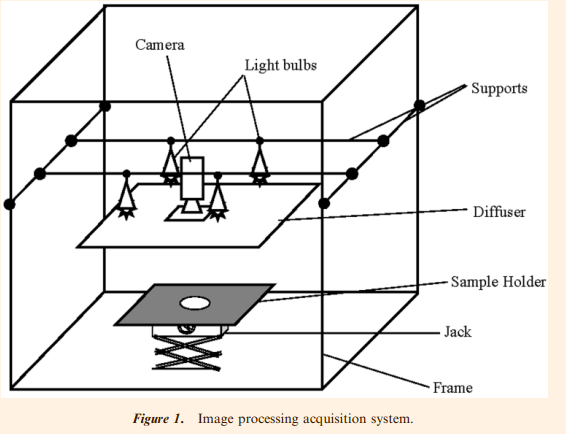
\includegraphics[width=0.5\linewidth]{imgs/1}
	\caption{}
	\label{fig:1}
\end{figure}

Twodifferent pictures were taken for each product after manually rotating the product 90. The volume (V) and surface area (S) of the objectwere computed as the sum of the volumes and, respectively, surface areas ofthe elementary cones as follows:

\end{document}
